% This example is meant to be compiled with lualatex or xelatex
% The theme itself also supports pdflatex
\PassOptionsToPackage{unicode}{hyperref}
\documentclass[aspectratio=1610, 9pt]{beamer}

% Load packages you need here
\usepackage[american]{babel}

\usepackage[autostyle]{csquotes}


\usepackage{amsmath}
\usepackage{amssymb}
\usepackage{mathtools}
\usepackage{xfrac}

\usepackage{tikz}
\usetikzlibrary{arrows.meta}
\usepackage[
  separate-uncertainty=true,
  per-mode=symbol-or-fraction,
]{siunitx}

% nice tables
\usepackage{tabularray}
\usepackage[outputdir=build]{minted}

% colors
\usepackage{xcolor}
\definecolor{lightblue}{RGB}{0, 152, 195}
\definecolor{darkblue}{RGB}{6, 17, 45}
\definecolor{apps}{RGB}{136, 181, 91}

\usepackage{hyperref}
\usepackage{bookmark}

% load the theme after all packages

\usetheme[dark]{tudo}

% Put settings here, like
\unimathsetup{
  math-style=ISO,
  bold-style=ISO,
  nabla=upright,
  partial=upright,
  mathrm=sym,
}

\title{ctapipe -- Prototype Open Event Reconstruction Pipeline for the Cherenkov Telescope Array}
\author[M.~Linhoff]{\emph{Maximilian Linhoff}, Lukas Nickel, Noah Biederbeck for the CTA Consortium and Observatory}
\institute[{%
  \begin{tikzpicture}[baseline=(node.south)]
    \node[text width=5cm, align=right] (node) at (0, 0) {Astroparticle Physics\\WG Rhode \& Elsässer};
  \end{tikzpicture}
}]{Supported by the DFG (SFB 876 \& 1491) and the BMBF (ErUM Pro CTA-D)}
\titlegraphic{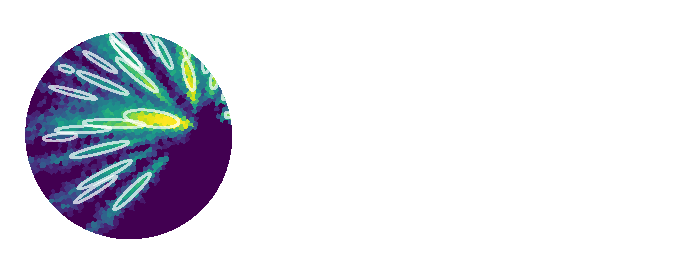
\includegraphics[height=0.4\textheight]{ctapipe-logo-dark.pdf}}
\date{2023-03-22}


\begin{document}

\maketitle

\begin{frame}{The Cherenkov Telescope Array Observatory}
  \begin{columns}[onlytextwidth, c]%
    \begin{column}{0.75\textwidth}%
      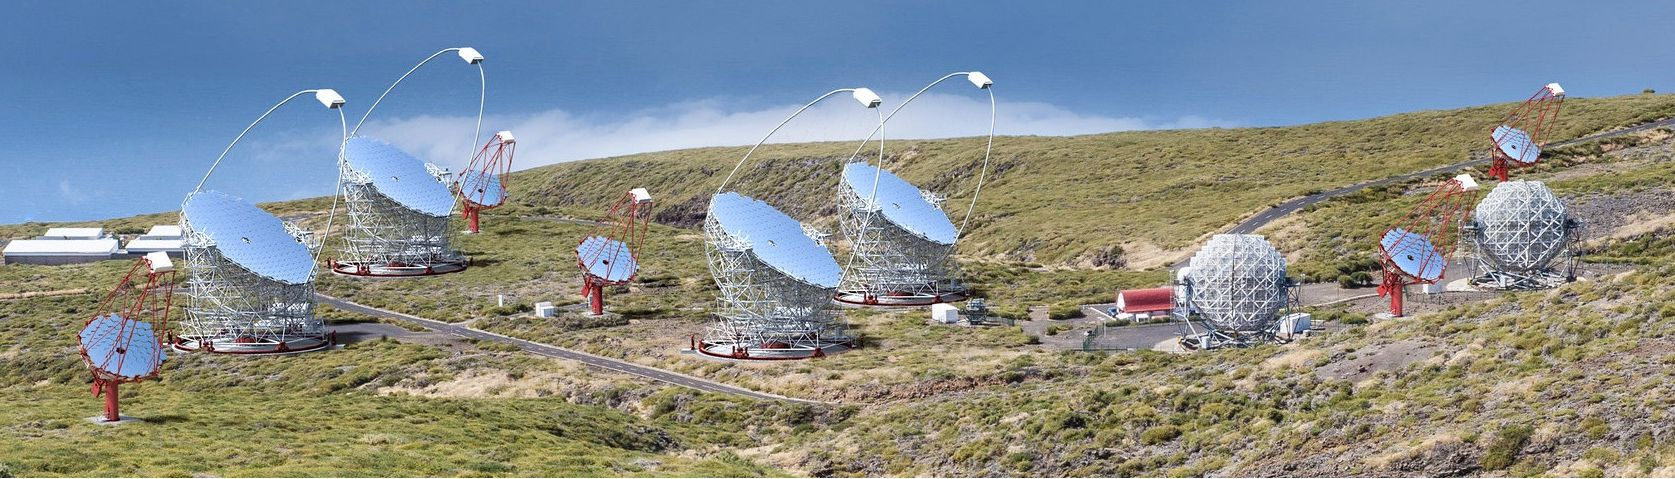
\includegraphics[width=\linewidth]{images/cta_north.jpg}
    \end{column}%
    \hfill%
    \begin{column}{0.24\textwidth}%
      CTA North (ORM, La Palma) \\
      4 LSTs, 9 MSTs (Alpha)\\
      LST-1 observing since 2018
    \end{column}%
  \end{columns}
  \medskip
  \begin{columns}[onlytextwidth, c]%
    \begin{column}{0.24\textwidth}%
      CTA South (ORM, La Palma) \\
      14 MSTs, 37 SSTs  (Alpha)\\
    \end{column}%
    \hfill%
    \begin{column}{0.74\textwidth}%
      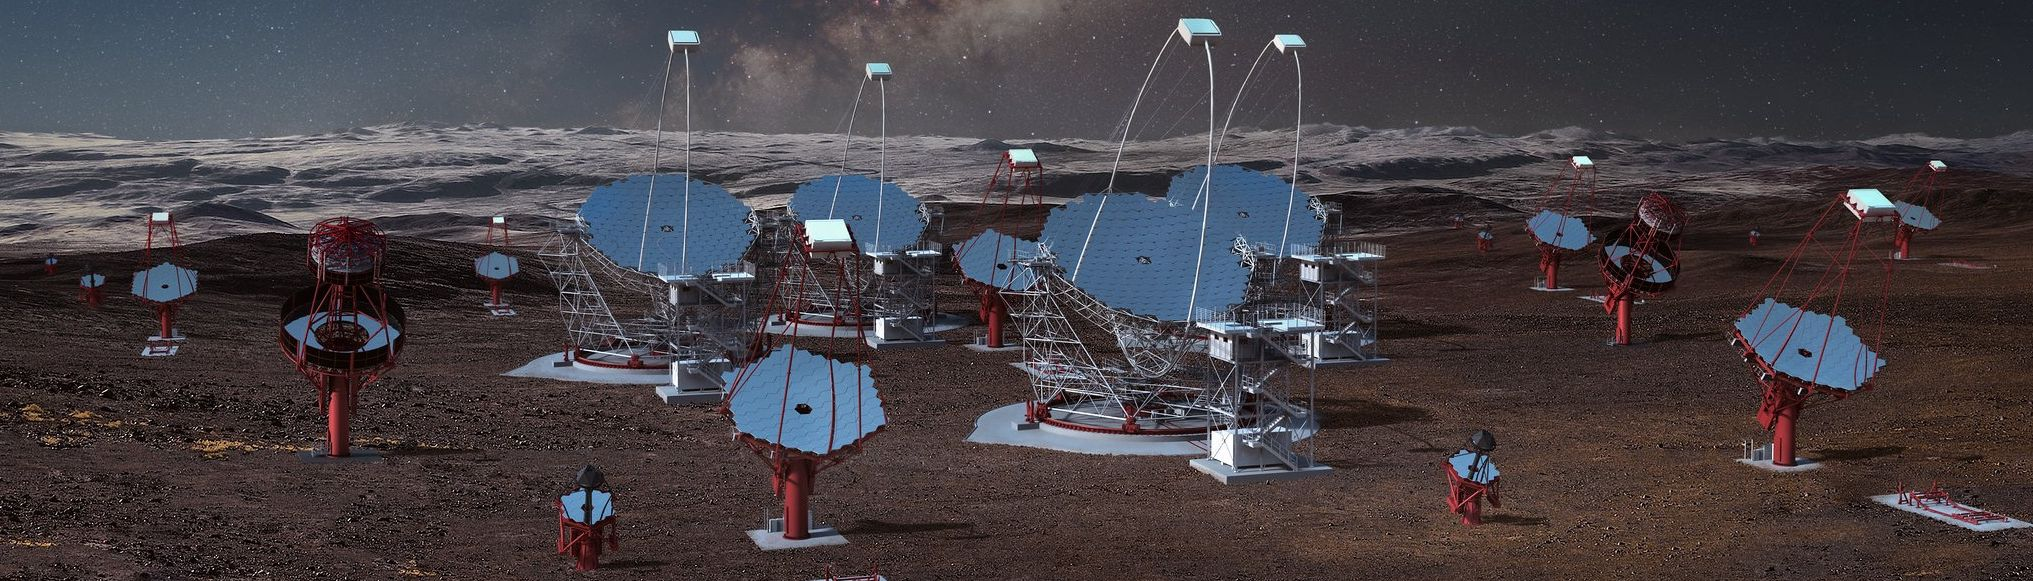
\includegraphics[width=\linewidth]{images/cta_south.jpg}
    \end{column}%
  \end{columns}
  \medskip

  \begin{center}
    \textasciitilde 30\,PB / year of archived raw data | High Level Reconstructed Data Published after Proprietary Period
  \end{center}
\end{frame}

\begin{frame}{ctapipe}
  \begin{itemize}
    \item Library and Tools for IACT event reconstruction
    \item Core library of the CTAO Data Processing and Preservation System (DPPS)
    \item Open, community-based development steered by CTAO maintainers
    \item \href{https://github.com/cta-observatory/ctapipe}{github.com/cta-observatory/ctapipe}
    \item Current release: \texttt{v0.18.0} – 2023-02-09
      \href{https://doi.org/10.5281/zenodo.3372210}{
\includegraphics[height=2ex]{images/ctapipe_zenodo.pdf}}
      \href{https://pypi.org/project/ctapipe}{
\includegraphics[height=2ex]{images/ctapipe_pypi.pdf}}
      \href{https://anaconda.org/conda-forge/ctapipe}{
\includegraphics[height=2ex]{images/ctapipe_conda.pdf}}
  \end{itemize}
\end{frame}

\begin{frame}
  \resizebox{\textwidth}{!}{%
\begin{tikzpicture}
  \tikzset{arrow/.style={-{Triangle Cap}, line width=10pt, shorten >= 5pt, shorten <= 5pt}}
  \tikzset{lightbg/.style={fill=lightgray, rounded corners=0.5cm, inner sep=0.2cm}}

  \node[] (ctapipe) at (0, 0) {
\includegraphics[width=10cm]{logos/ctapipe_logo_square.png}};

  \node[anchor=east, lightbg] (astropy) at (-8, 4.5) {
\includegraphics[height=2cm]{logos/astropy.pdf}};
  \node[anchor=north west, yshift=-0.5cm] (sklearn) at (astropy.south west) {
\includegraphics[height=2cm]{logos/sklearn.pdf}};
  \node[anchor=north west, yshift=-0.5cm] (numpy) at (sklearn.south west) {
\includegraphics[height=2cm]{logos/numpy.pdf}};
  \node[anchor=north west, yshift=-0.5cm, lightbg] (scipy) at (numpy.south west) {
\includegraphics[height=2cm]{logos/scipy.png}};
  \node[anchor=north west, yshift=-0.5cm] (pytables) at (scipy.south west) {
\includegraphics[height=2cm]{logos/pytables.png}};
  \node[anchor=north west, yshift=-0.5cm, lightbg] (matplotlib) at (pytables.south west) {
\includegraphics[height=2cm]{logos/matplotlib.pdf}};

  \draw[arrow, color=lightblue] (astropy.east) to[out=0, in=120] (120:5cm);
  \draw[arrow, color=lightblue] (sklearn.east) to[out=0, in=150] (150:5cm);
  \draw[arrow, color=lightblue] (numpy.east) to[out=0, in=170] (170:5cm);
  \draw[arrow, color=lightblue] (scipy.east) to[out=0, in=190] (190:5cm);
  \draw[arrow, color=lightblue] (pytables.east) to[out=0, in=200] (210:5cm);
  \draw[arrow, color=lightblue] (matplotlib.east) to[out=0, in=200] (230:5cm);

  \node[rectangle, fill=lightblue, minimum width=4.5cm, minimum height=4.5cm, text=white, anchor=north east, xshift=-0.25cm, yshift=-1cm, align=center, text width=4cm] (algos) at (ctapipe.south) {\Huge Algorithms\\\Huge \strut python, \strut numpy, \strut scipy};
  \node[rectangle, fill=darkblue, minimum width=4.5cm, minimum height=4.5cm, text=white, anchor=north west, xshift=0.25cm, yshift=-1cm, align=center] (numba) at (ctapipe.south) {\Huge Algorithms\\\Large Jit Compiled using \\ 
\includegraphics[width=4cm]{logos/numba.pdf}};

  \draw[{Triangle Cap}-{Triangle Cap}, color=darkblue, line width=10pt] (algos.north) to[out=90, in=245] (245:5cm);
  \draw[{Triangle Cap}-{Triangle Cap}, color=darkblue, line width=10pt] (numba.north) to[out=90, in=295] (295:5cm);

  \node[rectangle, fill=apps, minimum width=4.5cm, text width=4.5cm, minimum height=4.5cm, text=white, anchor=south west, yshift=0.25cm, xshift=1cm, align=center, font=\fontsize{32}{32}\selectfont] (tools) at (ctapipe.east) {pipeline\\tools};
  % \node[rectangle, fill=apps, minimum width=4.5cm, text width=4.5cm, minimum height=4.5cm, text=white, anchor=north west, yshift=-0.25cm, xshift=1cm, align=center, font=\huge] (advanced) at (ctapipe.east) {advanced\\pipeline\\applications};
  \node[anchor=north, yshift=-2.5cm, fill=apps] (jupyter) at (tools.south) {
\includegraphics[width=4cm]{logos/jupyter.pdf}};

  \draw[{Triangle Cap}-{Triangle Cap}, color=apps, line width=10pt] (tools.west) to[out=180, in=25] (25:5cm);
  % \draw[{Triangle Cap}-{Triangle Cap}, color=apps, line width=10pt] (advanced.west) to[out=180, in=-25] (-25:5cm);
  \draw[{Triangle Cap}-{Triangle Cap}, color=apps, line width=10pt] (jupyter.west) to[out=135, in=-45] (-45:5cm);

  \node[anchor=west, color=red!60!yellow, font=\Huge, yshift=1cm, xshift=0.5cm, text width=4cm] (deploy) at (tools.north east) {CI, Release \& Deploy};
  \node[anchor=north] (conda) at (deploy.south) {
\includegraphics[width=4cm]{logos/conda.pdf}};
  \node[anchor=north, yshift=-0.5cm] (forge) at (conda.south) {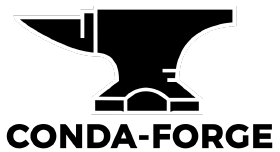
\includegraphics[width=4cm]{logos/conda-forge.png}};
  \node[anchor=north, yshift=-0.5cm] (pypi) at (forge.south) {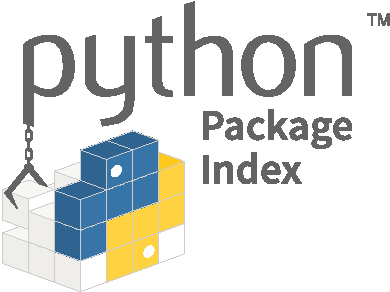
\includegraphics[width=4cm]{logos/pypi.pdf}};
  \node[anchor=north, yshift=-0.5cm] (pytest) at (pypi.south) {
\includegraphics[width=4cm]{logos/pytest.pdf}};
  \node[anchor=north, yshift=-0.5cm] (github) at (pytest.south) {
\includegraphics[width=4cm]{logos/github.pdf}};
\end{tikzpicture}
}

\end{frame}

\begin{frame}
  \begin{tikzpicture}
  \tikzset{datalevel/.style={thick, circle, draw, inner sep=2pt, minimum size=25pt}}
  \tikzset{analysis-step/.style={align=center, font=\footnotesize}}
  \tikzset{step-arrow/.style={-{Triangle Cap}, line width=5pt, shorten >= 5pt, shorten <= 5pt}}

    % raw data plot
    \node[] (R0Graph)   at (0.0, 0) {\includegraphics[height=1.75cm]{build/r0.pdf}};
    \node[] (R1Graph)   at (2.5, 0) {\includegraphics[height=1.75cm]{build/r1.pdf}};
    \node[] (DL0Graph)  at (5.0, 0) {\includegraphics[height=1.75cm]{build/dl0.pdf}};

    \node[] (DL1ImageGraph)   at (10.0, 0.0) {\includegraphics[height=2.5cm]{build/dl1a.pdf}};
    \node[] (DL1CleanGraph) at (10.0, -5) {\includegraphics[height=2.5cm]{build/dl1a_clean.pdf}};

    % Param table
    \node [font=\scriptsize] (DL1bTable) at (1.5, -6) {
      \SetTblrInner{rowsep=0pt, colsep=2pt}
      \begin{tblr}{
          colspec={rrrrcr},
          row{1}={font=\bfseries},
      }
        event &  hillas\_intensity & hillas\_width  & hillas\_length  & $\cdots$ & concentration\_cog \\
          0 &  1253.1    &  0.15  &   0.52  & $\cdots$ & 0.35 \\
          2 &   321.3    &  0.05  &   0.12  & $\cdots$ & 0.42 \\
          5 &   512.7    &  0.08  &   0.19  & $\cdots$ & 0.45 \\
      \end{tblr}
    };

    % Reconstruction table
    \node[font=\scriptsize] (DL2Table) at (1, -3.5) {
        \SetTblrInner{rowsep=0pt, colsep=2pt}
        \begin{tblr}{
            colspec={rrrrrr},
            row{1}={font=\bfseries},
        }
        event & energy & gammaness &    ra &    dec &        time \\
              &        &           &   deg &    deg &        mjd  \\
            0 &   1500 &      0.82 &  83.6 &   22.1 & 59024.63123 \\
            2 &    400 &      0.73 &  83.5 &   21.9 & 59024.64183 \\
            5 &    680 &      0.92 &  83.7 &   22.0 & 59024.67093 \\
        \end{tblr}
    };

    \node [datalevel, color=gray, anchor=north]    (R0)   at (R0Graph.south)   {R0};
    \node [datalevel, color=gray, anchor=north]    (R1)   at (R1Graph.south)   {R1};
    \node [datalevel, anchor=north]                (DL0)  at (DL0Graph.south) {DL0};
    \node [datalevel, anchor=east, xshift=1.3cm, yshift=-0.1cm] (DL1Image) at (DL1ImageGraph.south west) {DL1a};
    \node [datalevel, anchor=east, xshift=0.7cm, yshift=-0.1cm] (DL1Clean) at (DL1CleanGraph.north west) {DL1a};
    \node [datalevel, anchor=west] (DL1b) at (DL1bTable.east) {DL1b};
    \node [datalevel, anchor=west] (DL2)  at (DL2Table.east) {DL2};

    \draw[step-arrow, color=gray] (R0.east) -- (R1.west)  node [analysis-step, midway, below, text width=2cm] {Low-Level\\Calibration};
    \draw[step-arrow, color=gray] (R1.east) -- (DL0.west)  node [analysis-step, midway, below, text width=2cm] {Data Volume\\ Reduction};
    \draw[step-arrow] (DL0.east) -- (DL1Image.west)  node [analysis-step, midway, below, yshift=-0.15cm] {Pulse Extraction};
    \draw[step-arrow] (DL1Image.south east) to[out=315, in=45]  node [analysis-step, midway, right, xshift=0.2cm] {Image Cleaning} (DL1Clean.north east); 
    \draw[step-arrow] (DL1Clean.south) to[bend left] node [analysis-step, midway, above, xshift=-0.7cm, yshift=0.3cm] {Parametrization} (DL1b.east);
    \draw[step-arrow] (DL1b.110) -- (DL2.south east)  node [analysis-step, midway, left, yshift=-0.2cm] {Reconstruction};

\end{tikzpicture}

\end{frame}

\begin{frame}{Release 0.18}
  \begin{itemize}
    \item New reconstruction methods based on sklearn
      \begin{itemize}
        \item Particle Classification (Gamma / Hadron)
        \item Primary Energy
        \item Disp-Method for direction reconstruction
      \end{itemize}
    \item CLI-Applications to train / apply models
    \item Plugin system also for reconstruction methods
  \end{itemize}

  \bigskip
  \begin{center}
    \large
    $\Rightarrow$ ctapipe now able to produce fully reconstructed DL2 event data
  \end{center}
\end{frame}

\begin{frame}{Data Format}
  \begin{itemize}
    \item Plugin-System for input data
    \item HDF5 for output, including rich metadata, compression, transformations
    \item Utilities for bulk loading data into  \texttt{astropy.table.Table}s
  \end{itemize}
\end{frame}

\begin{frame}{Standard Workflow DL0 → DL2}
\end{frame}

\begin{frame}{Public DL1 / DL2 Data Release}
  \begin{itemize}
    \item Newly released dataset on Zenodo
    \item Simulated gamma-ray and proton events at DL1 (including images) and DL2 (only geometry) 
    \item 50 GB (size limit of Zenodo)
    \item ca.~ 500\,000 successfully reconstructed array events for each particle type
    \item Well-suited for machine learning studies at all levels
    \item Public, cite-able dataset: \href{https://doi.org/10.5281/zenodo.7298568}{
\includegraphics[height=2ex]{./images/public_data_zenodo.pdf}}

    \item Everything shown uses this dataset, full workflow / talk source available here: \\
      \href{https://github.com/maxnoe/ctapipe-dpg-2023}{github.com/maxnoe/ctapipe-dpg-2023}
  \end{itemize}
\end{frame}

\end{document}
